\graphicspath{ {./content/method/figures/} }
\onecolumn
\begin{landscape}

\begin{figure*}[Ht]
  \centering
  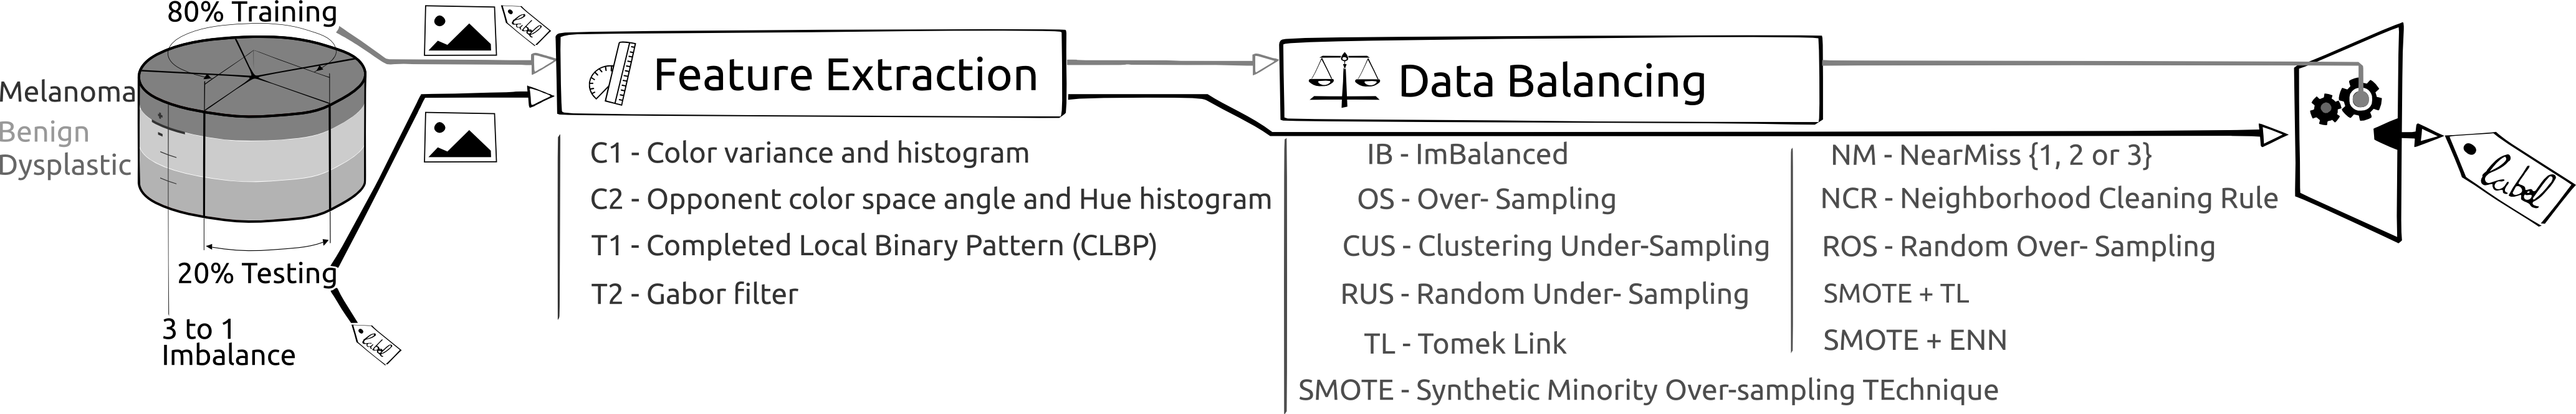
\includegraphics[width=1.4\textwidth]{method.png}
  \caption{Framework outline}
	\label{fig:schema}
\end{figure*}

\begin{table*}
\caption{The obtained results with different balancing techniques for color and texture features using a \acs*{rf} classifier. The first and second highest results for each feature set are highlighted in dark and lighter gray colors, respectively.}
\centering
\resizebox{1.42\textwidth}{!}{
\begin{tabular}{l cccccc		cccccc		cccccc}
\toprule
Features &  \multicolumn{6}{l}{Color}& \multicolumn{6}{l}{Texture} & \multicolumn{6}{l}{Combined}\\
  \cmidrule(r){2-7}  \cmidrule(r){8-13}  \cmidrule(r){14-19}  
		   & \multicolumn{2}{c}{$C_{1}$}& \multicolumn{2}{c}{$C_{2}$}& \multicolumn{2}{c}{$C_{1,2}$}& \multicolumn{2}{c}{$T_{1}$} &  \multicolumn{2}{c}{$T_{2}$} & \multicolumn{2}{c}{$T_{1,2}$}& \multicolumn{2}{c}{$T_{1},C_{1,2}$}& \multicolumn{2}{c}{$T_{2},C_{1,2}$}& \multicolumn{2}{c}{$T_{1,2},C_{1,2}$}\\ 
  \cmidrule(r){2-3}  \cmidrule(r){4-5} \cmidrule(r){6-7} \cmidrule(r){8-9} \cmidrule(r){10-11} \cmidrule(r){12-13} \cmidrule(r){14-15} \cmidrule(r){16-17} \cmidrule(r){18-19} 
  Balancing techniques & \makebox[0.5cm][l]{\acs*{se}}& \makebox[0.5cm][l]{\acs*{sp}} & \makebox[0.5cm][l]{\acs*{se}} & \makebox[0.5cm][l]{\acs*{sp}} & \makebox[0.5cm][l]{\acs*{se}} &\makebox[0.5cm][l]{\acs*{sp}} &\makebox[0.5cm][l]{\acs*{se}} &\makebox[0.5cm][l]{\acs*{sp}} &\makebox[0.5cm][l]{\acs*{se}} & \makebox[0.5cm][l]{\acs*{sp}} &\makebox[0.5cm][l]{\acs*{se}} &\makebox[0.5cm][l]{\acs*{sp}} & \makebox[0.5cm][l]{\acs*{se}} &\makebox[0.5cm][l]{\acs*{sp}} &\makebox[0.5cm][l]{\acs*{se}} &\makebox[0.5cm][l]{\acs*{sp}}& \makebox[0.5cm][l]{\acs*{se}} &\makebox[0.5cm][l]{\acs*{sp}}  \\ \midrule
\multicolumn{19}{c}{}\\[-2.2ex]  
\multicolumn{1}{c}{IB} & 52.5 & 89.6 & 75.0 & 88.7 & 71.2 & 87.5 & 38.7 & 91.7 & 60.0 & 96.2 & 66.2 & 93.7 &73.7 & 89.6 & 71.2 & 89.6 & 71.2 & 92.5\\
\multicolumn{19}{c}{}\\[-2.2ex]  
\midrule \midrule
\multicolumn{19}{c}{}\\[-2.2ex]  
\multicolumn{1}{c}{\acs*{os}} &\cellcolor[gray]{0.6}93.7 &\cellcolor[gray]{0.6}66.7 & 80.0 & 86.2 & 82.5 & 87.1  & 43.7 &83.7 &\cellcolor[gray]{0.6}72.5 &\cellcolor[gray]{0.6}90.0 & 70.0 & 91.7  & 77.5 & 87.1 & 81.2  &88.3 & 78.7 & 88.3  \\
\multicolumn{19}{c}{}\\[-2.2ex]  
\midrule \midrule
\multicolumn{19}{c}{}\\[-2.2ex]  
\multicolumn{1}{c}{\acs*{ros}} &55.0 & 80.8 & 80.0 & 84.2 & 72.5 &85.4 & 42.5 & 82.1 & 60.0 & 89.2 & 66.2 & 87.9 & 75.0 & 85.4 & 73.7 & 86.2 & 73.7 & 85.8\\
\multicolumn{19}{c}{}\\[-2.2ex]
\multicolumn{1}{c}{\acs*{smote}} & 60.0 & 82.5 & 78.7 & 84.6 & 75.0 & 70.0 & 56.2 & 74.2 & 61.2 & 87.5 & 84.2 & 87.1 & 78.7 & 85.0 &73.7 & 84.6 & 73.7 & 85.0 \\ 
\multicolumn{19}{c}{}\\[-2.2ex]
\hdashline \noalign{\vskip 3pt}
\multicolumn{19}{c}{}\\[-2.2ex]
\multicolumn{1}{c}{\acs*{rus}} & 72.5 & 72.9 & 86.2 & 80.0 & 78.7 & 80.0 & 67.5 & 53.3 &76.2 & 76.2 & 85.0 & 78.7 & 91.2 & 75.0 & 85.0 & 78.7 & 92.5 & 78.3\\
\multicolumn{19}{c}{}\\[-2.2ex]
\multicolumn{1}{c}{\acs*{tl}} & 51.2 & 86.2 & 76.2 & 87.9 & 67.5 & 88.3 & 37.5 & 87.9 & 65.0 & 90.4 & 68.7 & 91.7 & 73.7 & 88.7 & 63.7 & 90.0 & 72.5 & 91.2\\
\multicolumn{19}{c}{}\\[-2.2ex]
\multicolumn{1}{c}{\acs*{cus}} & 81.2 & 67.9 & 80.0 & 84.6 & 86.2 & 80.4 & 56.2 & 65.8 & 70.0 & 77.5 & 85.0 & 77.1 & 83.7 & 81.2 & 80.0 & 84.2 & 83.7 & 82.9\\
\multicolumn{19}{c}{}\\[-2.2ex]
\multicolumn{1}{c}{\acs*{nm1}} & 67.5 & 72.1 & 86.2 & 79.2 & 85.0 & 82.5 & 72.5 & 43.7 & 80.0 & 62.5 & 87.5 & 66.7 & 85.0 & 82.1 & 86.2 & 80.4 & 87.5 & 80.8\\
\multicolumn{19}{c}{}\\[-2.2ex]
\multicolumn{1}{c}{\acs*{nm2}} & 70.0 & 72.9 & 86.2 & 81.2 & 85.0 & 82.9 & 76.2 & 48.7 & 86.2 & 40.8 & 86.2 & 51.2 & \cellcolor[gray]{0.6}87.5 & \cellcolor[gray]{0.6}82.1   &\cellcolor[gray]{0.6}92.5 &\cellcolor[gray]{0.6}77.5 &\cellcolor[gray]{0.6}91.2 &\cellcolor[gray]{0.6}81.7\\
\multicolumn{19}{c}{}\\[-2.2ex]
\multicolumn{1}{c}{\acs*{nm3}} & 82.5 & 75.0 & 87.5 & 80.8 & 85.0 & 80.4 & 73.7 & 55.8 & 72.5 & 82.5 & 82.5 & 80.4 & 83.7 & 81.2 & 85.0 & 80.0 & 86.2 & 80.4\\
\multicolumn{19}{c}{}\\[-2.2ex]
\multicolumn{1}{c}{\acs*{ncr}} & 66.2 & 76.7 & \cellcolor[gray]{0.6} 87.5 &\cellcolor[gray]{0.6}81.2 & 85.0 & 82.1 & 67.5 & 67.9 & 75.0 & 85.8 & \cellcolor[gray]{0.6}82.5 & \cellcolor[gray]{0.6}83.3 &  86.2 &  81.7 & 82.5  & 85.0 & 83.7  & 85.4\\
\multicolumn{19}{c}{}\\[-2.2ex]
\hdashline \noalign{\vskip 3pt}
\multicolumn{19}{c}{}\\[-2.2ex]
\multicolumn{1}{c}{\acs*{smote} + \acs*{enn}} & 76.2 & 73.3 & 85.0 & 81.2 & 85.0 & 82.1 &\cellcolor[gray]{0.6} 81.2 &\cellcolor[gray]{0.6} 56.2 & 76.2 & 82.1 & 80.0 & 79.6 & 86.2 & 81.2 & 83.7 & 82.5 & 78.7 & 82.9\\
\multicolumn{19}{c}{}\\[-2.2ex]
\multicolumn{1}{c}{\acs*{smote} + \acs*{tl}} & 75.0 & 73.7 & 83.7 & 82.5 & \cellcolor[gray]{0.6}87.5 &\cellcolor[gray]{0.6}80.8 & 72.5 & 59.2 & 77.5 & 82.1 & 78.7 & 78.7 & 85.0 & 82.1 & 77.5 & 82.9 & 88.7 & 82.5\\
\multicolumn{19}{c}{}\\[-2.2ex]
\bottomrule
\end{tabular}
}
\label{tab:tab1}
\end{table*}

\normalsize \vfill
\end{landscape}
\twocolumn
